% Created 2015-06-10 Wed 10:39
\documentclass[11pt]{article}
\usepackage[utf8]{inputenc}
\usepackage[T1]{fontenc}
\usepackage{fixltx2e}
\usepackage{graphicx}
\usepackage{longtable}
\usepackage{float}
\usepackage{wrapfig}
\usepackage{rotating}
\usepackage[normalem]{ulem}
\usepackage{amsmath}
\usepackage{textcomp}
\usepackage{marvosym}
\usepackage{wasysym}
\usepackage{amssymb}
\usepackage{hyperref}
\tolerance=1000
\author{Patrick Guenthard}
\date{\today}
\title{README}
\hypersetup{
  pdfkeywords={},
  pdfsubject={},
  pdfcreator={Emacs 24.5.1 (Org mode 8.2.10)}}
\begin{document}

\maketitle
\tableofcontents

\section{Blog-CMS}
\label{sec-1}

\begin{itemize}
\item Small Blog-CMS
\item School Project at BBW
\end{itemize}

\subsection{Screenshots of the main page and the update page 2015-05-15}
\label{sec-1-1}
\subsubsection{main page}
\label{sec-1-1-1}
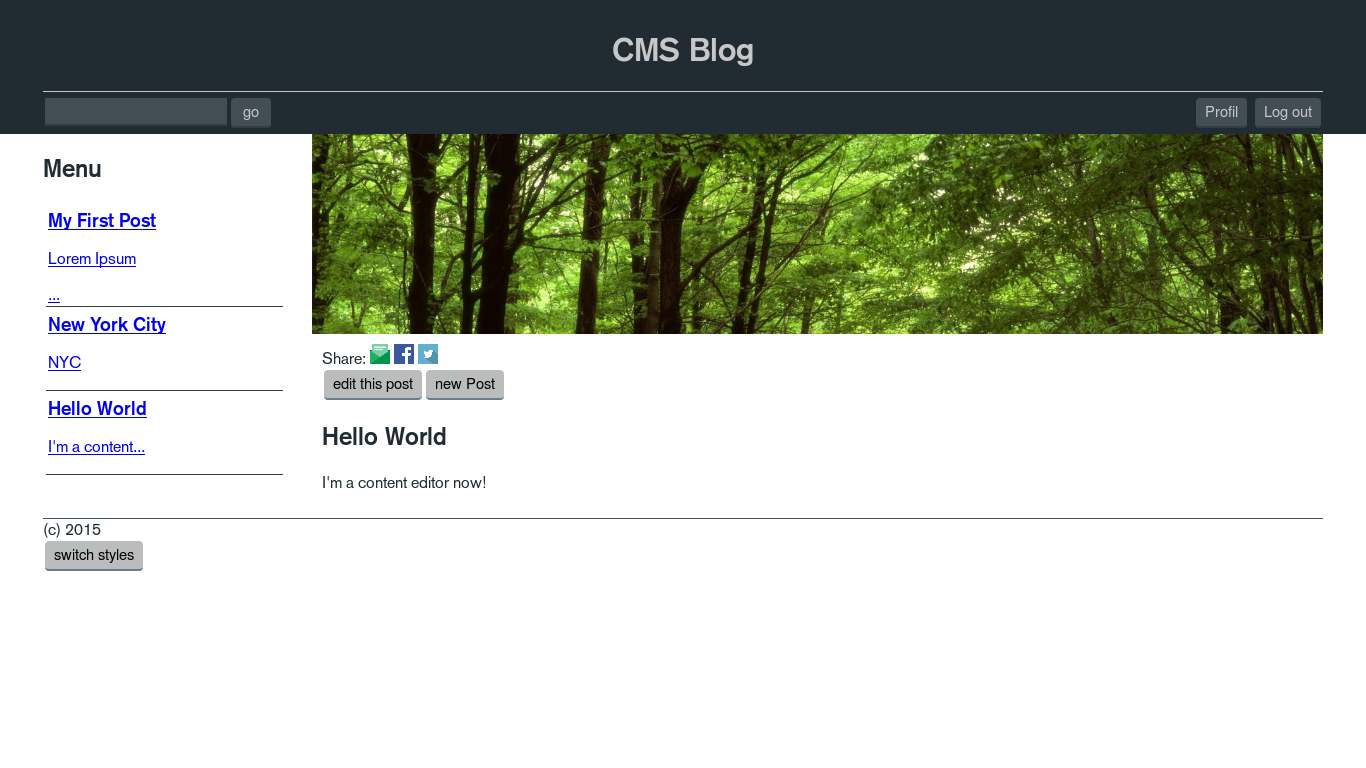
\includegraphics[width=.9\linewidth]{./info/img/screenshot-main-2015-05-15.png}

\subsubsection{update page}
\label{sec-1-1-2}
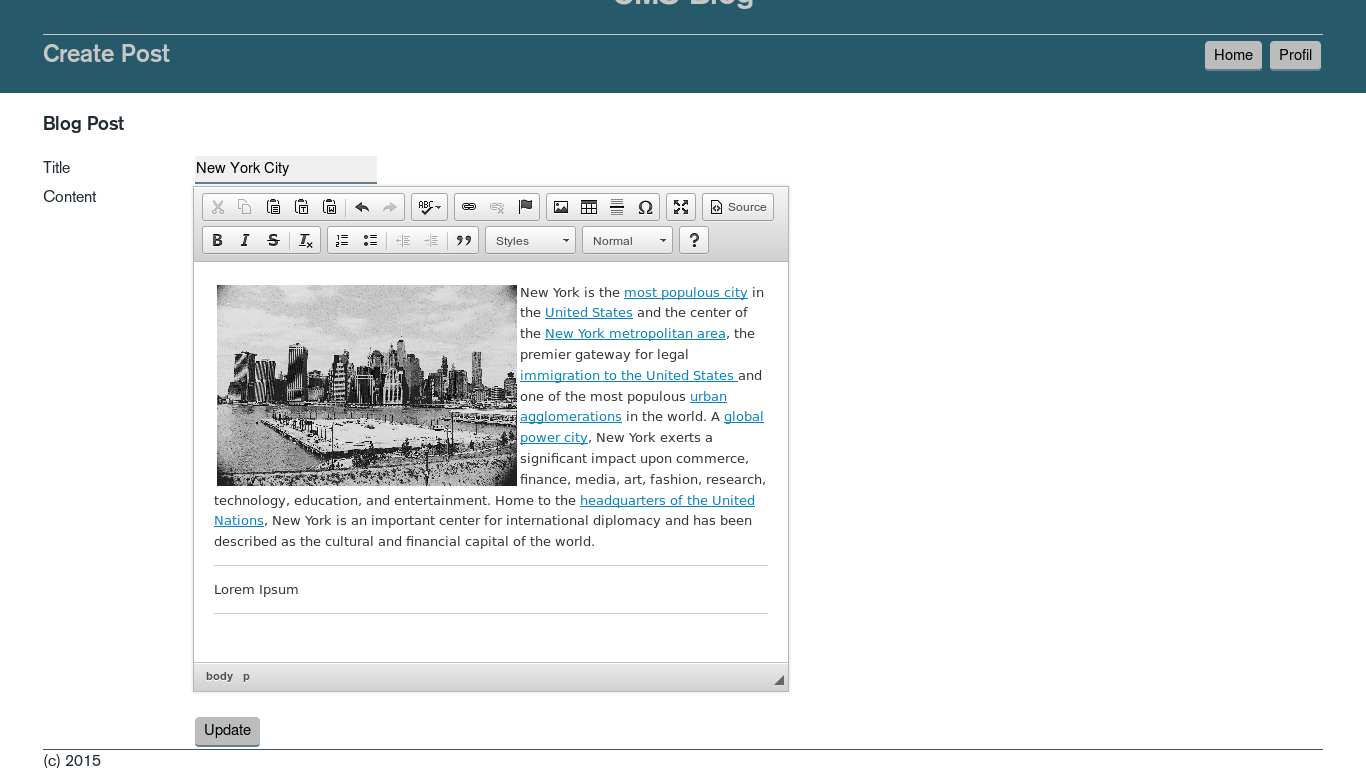
\includegraphics[width=.9\linewidth]{./info/img/screenshot-update-2015-05-15.png}

\subsection{Screenshot of the main page 2015-05-08}
\label{sec-1-2}
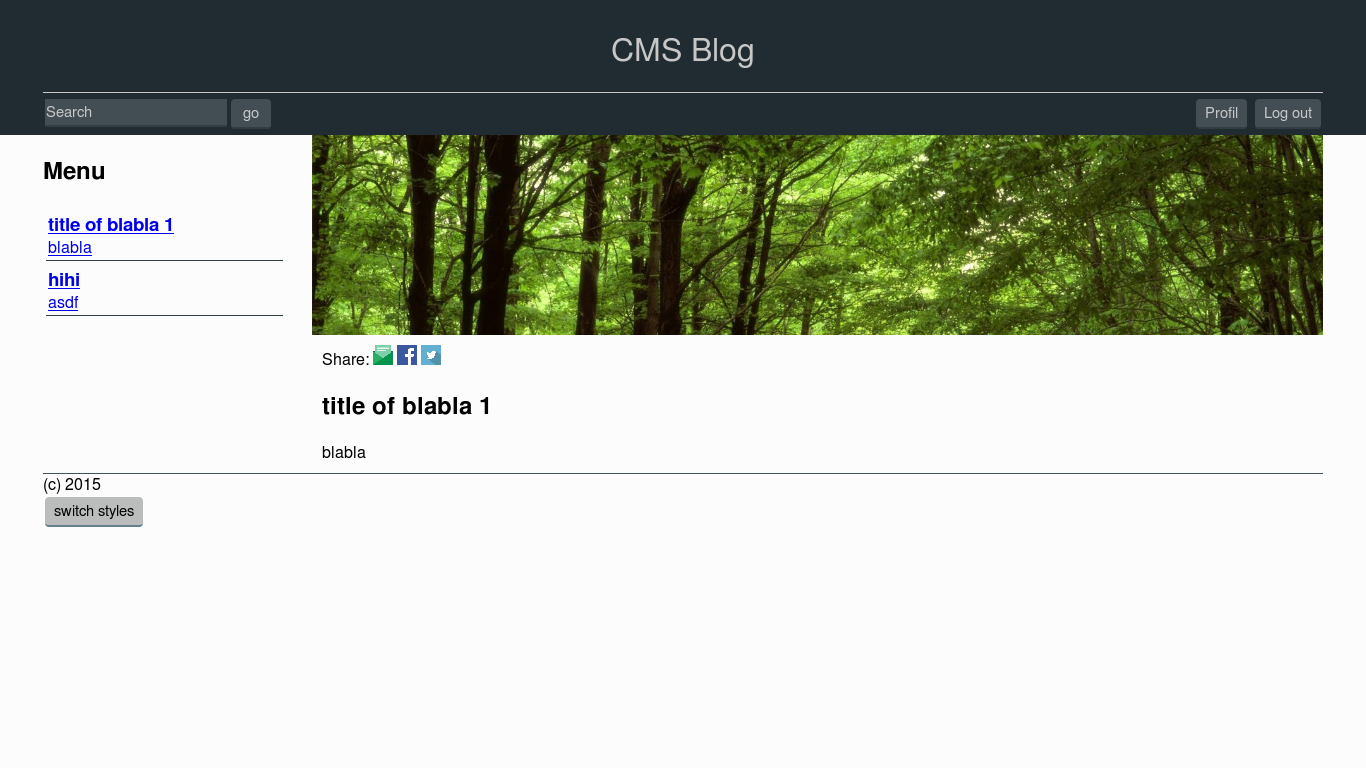
\includegraphics[width=.9\linewidth]{./info/img/screenshot-state-2015-05-08.png}
% Emacs 24.5.1 (Org mode 8.2.10)
\end{document}
